\chapter{DFA e NFA}
\section{DFA}
I DFA (Deterministic Final Automa) o \textbf{Automi a Stati Finiti Deterministici} un tipo di automa in grado
di accettare grammatiche di tipo 3 (Regolari).
\'E una quintupla definita come segue:
\begin{equation*}
    A={Q, \Sigma, \delta, q_0, F}    
\end{equation*}
Dove delta è una funzione che prende come input uno stato q e un simbolo
dell'alfabeto $\Sigma$ e restituisce uno stato.
\begin{equation*}
    \delta(q_0, a)=q_1
\end{equation*}
Nei DFA delta è una funzione totale, cioè tutte le combinazioni stato stringa sono
definite (nei NFA non è così).
%Inserire spiegazione lettere
\section{NFA}
I NFA (Non Deterministic Final Automa) o \textbf{Automi a Stati Finiti Non Deterministici} sono sempre definiti
come quintupla definita come segue:
\begin{equation*}
    A={Q, \Sigma, \delta, q_0, F}    
\end{equation*}
In questo caso la $\delta$ prende sempre un carattere e uno stato come input, ma
restituisce un sottoinsieme di Q, quindi un insieme di stati.
Questo significa che l'automa può assumere più stati in contemporanea, con un simbolo per
esempio posso andare in 2 stati diversi.
\paragraph*{Differenza tra NFA e DFA}L’unica
differenza tra un NFA e un DFA è quindi nel tipo di valore restituito da $\delta$: un insieme di
stati nel caso di un NFA e un singolo stato nel caso di un DFA.
\paragraph*{NFA e DFA, hanno la stessa potenza?} Sì, ogni NFA può essere convertito in un DFA, 
c'è da tenere in considerazione che gli NFA sono più compatti dei DFA in termini di rappresentazione
grafica.
\section{Epsilon NFA}
Un $\epsilon$ NFA è come un NFA che però può eseguire delle $\epsilon$-mosse,
cioè può andare da un stato a un altro senza consumare un simbolo della stringa
data in input.
Formalmente è sempre denotato come $A = (Q, \Sigma, \delta, q_0, F)$ dove tutti 
i componenti si interpretano come nel caso di un NFA, tranne $\delta$ che è una funzione
che richiede come argomenti:
\begin{itemize}
    \item Uno stato in Q
    \item un elemento di $\Sigma \cup \{\epsilon\}$, cioè un simbolo di input o il
    simbolo $\epsilon$. Si richiede che il simbolo di stringa vuota $\epsilon$ non sia
    un elemento dell'alfabeto $\Sigma$ (se no si fa confusione)
\end{itemize}

\definizione{Eclose(q)
\\ è l'insieme di stati di Q che possono essere raggiunti a partire da q facendo solo 
$\epsilon$-mosse, compreso q stesso.}
A livello pratico per $\epsilon$-chiudere uno
stato q si seguono tutte le $\epsilon$-transizioni uscenti da q, ripetendo poi l'operazione da tutti gli
stati raggiunti via via, fino a trovare tulli gli siati raggiungibili da q attraverso cammini
etichettati solo da $\epsilon$-transizioni.

\section{Conversione da NFA a DFA}
Per ogni NFA c'è un corrispondente DFA.
Per convertire un $\epsilon$-NFA a DFA è necessario costruire una tabella, 
prendo lo stato iniziale e ne faccio l'eclose, scrivo l'insieme di stati risultante (se presente
uno stato finale allora lo segno con un asterisco) e poi per ogni simbolo dell'alfabeto
faccio la $\delta$ (verifico in che stati l'automa si troverà dopo aver consumato il carattere) 
e l'eclose dell'insieme degli stati ottenuto, scrivo l'insieme di stati risultante 
(ancora una volta se presente uno stato finale allora segno con un asterisco tutto l'insieme).
Una volta eseguita la prima riga scrivo i nuovi insiemi di stati ottenuti (compreso quello vuoto)
nella prima colonna (quella degli insiemi degli stati) e proseguo fino a quando non trovo più nuovi
stati.
\\ Etichetto tutti gli insiemi degli stati e li scrivo come stati unici, verifico le transizioni che
mi portano da un insieme di stati all'altro e costruisco il DFA.

\section{Conversione da ER a Epsilon NFA}
Dovrò avere
\begin{enumerate}
    \item Esattamente uno stato accettante
    \item Nessun arco entrante nello stato iniziale
    \item Nessun arco uscente dallo stato accettante
\end{enumerate}
%Completare sto casino
\section{Conversione da Epsilon NFA a ER}
\'E sempre possibile convertire una ER in un $\epsilon$-NFA.
Si tratta di un processo piuttosto intuitivo, qui di seguito la conversione in
$\epsilon$-NFA della seguente ER:
\begin{equation*}
    (0 + 1)* 1(0 + 1) 
\end{equation*}
\begin{center}
    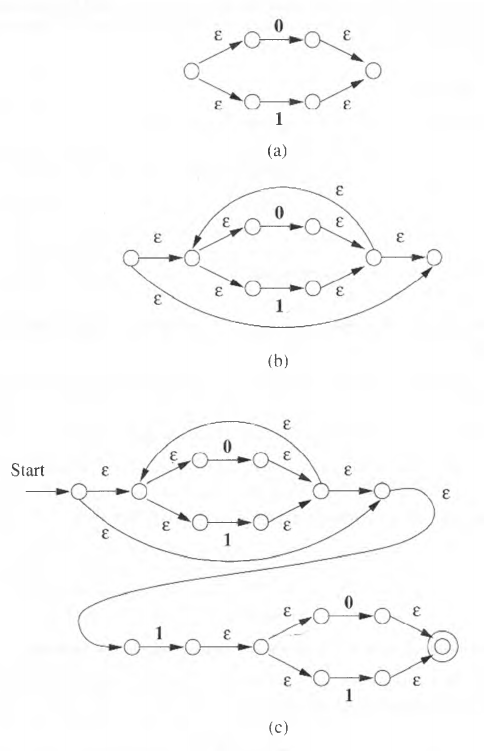
\includegraphics[width=50mm, scale=0.5]{img/er_to_nfa.png}
\end{center}
\section{Pumping Lemma}
Il Pumping lemma è un teorema che ci permette di dimostrare che un linguaggio non è regolare.
%Completare definizione